%%%%%%%%%%%%%%%%%%%%%%%%%%%%%%%%%%%%%%%%%
% Short Sectioned Assignment LaTeX Template Version 1.0 (5/5/12)
% This template has been downloaded from: http://www.LaTeXTemplates.com
% Original author:  Frits Wenneker (http://www.howtotex.com)
% License: CC BY-NC-SA 3.0 (http://creativecommons.org/licenses/by-nc-sa/3.0/)
%%%%%%%%%%%%%%%%%%%%%%%%%%%%%%%%%%%%%%%%%

%----------------------------------------------------------------------------------------
%	PACKAGES AND OTHER DOCUMENT CONFIGURATIONS
%----------------------------------------------------------------------------------------

\documentclass[paper=a4, fontsize=11pt]{scrartcl} % A4 paper and 11pt font size

% ---- Entrada y salida de texto -----

\usepackage[T1]{fontenc} % Use 8-bit encoding that has 256 glyphs
\usepackage[utf8]{inputenc}
%\usepackage{fourier} % Use the Adobe Utopia font for the document - comment this line to return to the LaTeX default

% ---- Idioma --------

\usepackage[spanish, es-tabla]{babel} % Selecciona el español para palabras introducidas automáticamente, p.ej. "septiembre" en la fecha y especifica que se use la palabra Tabla en vez de Cuadro

% ---- Otros paquetes ----

\usepackage{amsmath,amsfonts,amsthm} % Math packages
%\usepackage{graphics,graphicx, floatrow} %para incluir imágenes y notas en las imágenes
\usepackage{graphics,graphicx, float} %para incluir imágenes y colocarlas

% Para hacer tablas comlejas
%\usepackage{multirow}
%\usepackage{threeparttable}

%\usepackage{sectsty} % Allows customizing section commands
%\allsectionsfont{\centering \normalfont\scshape} % Make all sections centered, the default font and small caps

\usepackage{fancyhdr} % Custom headers and footers
\usepackage{url}
\usepackage{hyperref}
\pagestyle{fancyplain} % Makes all pages in the document conform to the custom headers and footers
\fancyhead{} % No page header - if you want one, create it in the same way as the footers below
\fancyfoot[L]{} % Empty left footer
\fancyfoot[C]{} % Empty center footer
\fancyfoot[R]{\thepage} % Page numbering for right footer
\renewcommand{\headrulewidth}{0pt} % Remove header underlines
\renewcommand{\footrulewidth}{0pt} % Remove footer underlines
\setlength{\headheight}{13.6pt} % Customize the height of the header

\numberwithin{equation}{section} % Number equations within sections (i.e. 1.1, 1.2, 2.1, 2.2 instead of 1, 2, 3, 4)
\numberwithin{figure}{section} % Number figures within sections (i.e. 1.1, 1.2, 2.1, 2.2 instead of 1, 2, 3, 4)
\numberwithin{table}{section} % Number tables within sections (i.e. 1.1, 1.2, 2.1, 2.2 instead of 1, 2, 3, 4)

\setlength\parindent{0pt} % Removes all indentation from paragraphs - comment this line for an assignment with lots of text

\newcommand{\horrule}[1]{\rule{\linewidth}{#1}} % Create horizontal rule command with 1 argument of height

\usepackage{booktabs}




%----------------------------------------------------------------------------------------
%	TÍTULO Y DATOS DEL ALUMNO
%----------------------------------------------------------------------------------------

\title{	
\normalfont \normalsize 
\textsc{{\bf Aprendizaje Automático (2014-2015)} \\ Grado en Ingeniería Informática \\ Universidad de Granada} \\ [25pt] % Your university, school and/or department name(s)
\horrule{0.5pt} \\[0.4cm] % Thin top horizontal rule
\huge Práctica 3 \\ % The assignment title
\horrule{2pt} \\[0.5cm] % Thick bottom horizontal rule
}

\author{Ignacio Martín Requena} % Nombre y apellidos

\date{\normalsize\today} % Incluye la fecha actual

%----------------------------------------------------------------------------------------
% DOCUMENTO
%----------------------------------------------------------------------------------------
\usepackage{graphicx}
\usepackage{listings}
\usepackage{color}
\definecolor{gray97}{gray}{.97}
\definecolor{gray75}{gray}{.75}
\definecolor{gray45}{gray}{.45}
 

\lstset{ frame=Ltb,
     framerule=0pt,
     aboveskip=0.5cm,
     framextopmargin=3pt,
     framexbottommargin=3pt,
     framexleftmargin=0.4cm,
     framesep=0pt,
     rulesep=.4pt,
     backgroundcolor=\color{gray97},
     rulesepcolor=\color{black},
     %
     stringstyle=\ttfamily,
     showstringspaces = false,
     basicstyle=\small\ttfamily,
     commentstyle=\color{gray45},
     keywordstyle=\bfseries,
     %
     numbers=left,
     numbersep=15pt,
     numberstyle=\tiny,
     numberfirstline = false,
     breaklines=true,
   }
 


\lstdefinestyle{consola}
   {basicstyle=\scriptsize\bf\ttfamily,
    backgroundcolor=\color{gray75},
   }
 
\lstdefinestyle{C}
   {language=C,
   }



\begin{document}

\maketitle % Muestra el Título

\newpage %inserta un salto de página

\tableofcontents % para generar el índice de contenidos

\listoffigures

%\listoftables

\newpage



%----------------------------------------------------------------------------------------
%	Cuestion 1
%----------------------------------------------------------------------------------------

\section{Cuestionario}


\subsection{Suponga que dispone de una muestra i.i.d para estudiar la predicción del valor de una variable Y para un valor dado del predictor X.  Suponga que elige al azar uno de los métodos estudiados. ¿Cómo podríamos estimar la desviación típica de nuestra predicción? Dar todos los detalles de cada paso.}

Cogeriamos un subconjunto de datos de training y construiriamos el modelo a partir de este, a continuación calculariamos la media que el modelo ha generado pasandole el conjunto de test y obteniendo los resultados del mismo. Una vez obtenida la media aritmética calcularíamos la desviación típica con la fórmula:


\subsection{Describir que problema resuelve y cuál es el fundamento de la técnica de Validación Cruzada de k-partes (k-CV) y porque debe de funcionar. }

Al usar validación cruzada evitas que la muestra de train tenga datos ``especiales'' y obtengamos un modelo poco ajustado con la realidad. 

Al hacer validación cruzada, de alguna manera cogemos todo el conjunto de muestras como train menos una porción del mismo que la usaremos como test y asi con tantas conbinaciones como especifique el valor de K. 

Es decir, resuelve el problema de que cojamos un conjunto con muestras poco representativas.

\subsection{Describir las ventajas y desventajas de usar k-CV respecto de usar una aproximación basada en un conjunto de validación o en Leave-One-Out (LOO).}

\begin{itemize}

\item \textbf{Ventajas KCV}: El tiempo de computo con respecto a LOO es menor, asegura que test y training estarán mas equilibrados y obtenemos mejor error de test respecto a los otros modelos.

\item \textbf{Desventajas KCV}:  LOO hace que el modelo aprenda de mas muestras que en KCV, KCV es mas difícil de implementar frente a un solo conjunto de validación, hay un error de test variable porque pueden caer muestras poco representativas.


\end{itemize}

\subsection{¿En que beneficia la combinación de múltiples clasificadores frente al uso de un único clasificador? Justificar la respuesta}

Al usar multiples clasificadores obtenemos una mayor capacidad de contraste debido a la mayor informacion que poseemos sobre que clasificadores funcionan mejor sobre el modelo. A demás el uso de multiples clasificadores hace que tengamos mas liberta de modelizacion.

\subsection{¿Qué es y que aporta el predictor Random Forest frente al uso de  Bagging con árboles?
Justificar la respuesta.}

Random Forest esta construido sobre la ídea de bagging pero además también aporta una mejora ya que construye árboles no correlados.\\

Si existe un predictor muy fuerte en el conjunto de datos entonces muchos de ellos usarán dicho predictor para la primera partición.\\

El promedio de cantidades altamente correladas no reduce mucho su varianza y por tanto “random forest” correla los árboles de bagging para obtener una mayor reducción en varianza.\\


\subsection{Si tenemos dos métodos que son capaces de separar linealmente un problema de dos clases y uno de ellos es SVM-lineal. ¿Hay alguna razón que nos llevarían a preferir la técnica SVM frente al otro método? Justificar la respuesta}

Si hay una clara diferenciación entre los datos de una clase y de otra sería mejor tomar el metodo SVM-lineal, ya que no se ``sobreajusta'' tanto a las muestras como el modelo plenamente lineal, si no que traza una frontera minima y, de alguna manera, consigue encontrar la zona bajo la cual las muestras se dividen.

\subsection{¿Cuáles son las razones principales para usar técnicas de núcleo en un problema dado? Describir los casos y justificar la respuesta.}

Las tecnicas de núcleo son buenas para tener libertad a la hora de ajustar el modelo. Por ejemplo el Kernel radial nos da la posibilidad de definir un modelo a partir de la definición de un radio a partir del cual se situa la frontera de clasificación. Estas técnicas yo las usaria para problemas que necesiten un modelo algo diferente al resto.

\subsection{En un laboratorio de biológicos se procesan muestras de material genético para obtener un  modelo de predicción de cáncer. Debido al coste de procesamiento solo se pueden procesar un bajo número de muestras, sin embargo cada muestra proporciona un vector de variables de considerable longitud. Los investigadores son capaces de identificar que variables son relevantes  como predictores y cuales como predicción, pero no saben que técnica sería más conveniente aplicar en este caso. Discutir el problema y proponer y justificar soluciones adecuadas desde el punto de vista metodológico}

Eligiría un modelo que realizara pocas operaciones pero que fuera efectivo, ya que al tener tantisimas variables, un modelo como SVM podría tardar mucho en realizarse.

Un buen modelo podría ser validación cruzada o regresión logística. Validación cruzada con un modelo de clasificación por refresión logística nos daría buenos resultados sobre este conjunto de datos.


\section{Ejercicios de implementacion}

%----------------------------------------------------------------------------------------
%	Cuestion 1
%----------------------------------------------------------------------------------------
\subsection{Usar el conjunto de datos OJ que es parte del paquete ISLR}

\subsubsection{Crear un conjunto de entrenamiento conteniendo una muestra aleatoria de 800 observaciones, y un conjunto de test conteniendo el resto de las observaciones. Ajustar un clasificador SVM (con núcleo lineal) a los datos de entrenamiento usando cost=0.01, con “Purchase” como la respuesta y las otras variables como predictores.}

La salida que R nos muestra una vez ajustado el clasificador SVM es la siguiente:

\begin{figure}[H]
\centering
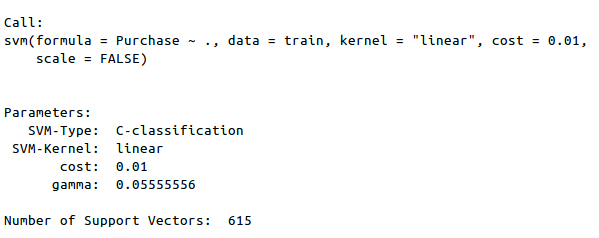
\includegraphics[scale=0.60]{ej1-1.png}
\caption{Salida R SVN nucleo lineal}
\label{}
\end{figure}

Como podemos ver R nos especifica que es de tipo clasificacion y con un nucleo lineal, que tiene un costo de 0.01 (por lo que al ser pequeño los margenes seran anchos y muchos vectores estaran en el margen) y un margen de hiperplanos de 0.0555

\subsubsection{Usar la función summary() para producir un resumen estadístico, y describir los resultados obtenidos. ¿Cuáles son las tasas de error de “training” y “test”?}

\begin{figure}[H]
\centering
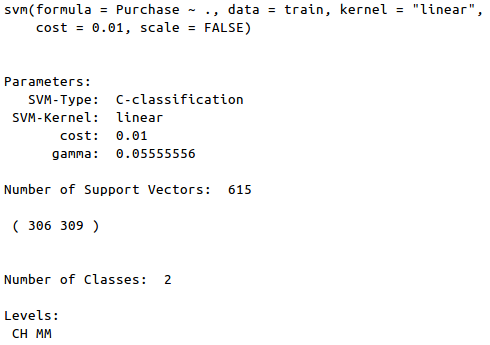
\includegraphics[scale=0.50]{ej1-2.png}
\caption{Salida R SVN nucleo lineal (summary)}
\label{}
\end{figure}

Además de lo comentado en el apartado anterior la funcion summary también nos muestra el número de support vectors y como están divididos en el modelo de clasificación, el numero de clases y los niveles.\\

En cuanto a la distribucion de los vectores se puede ver que es equilibrada ( 306 309 ), por lo que es posible que nuestro modelo sea bueno.

La tasa de error de train es del 26,25\% y la de test de 26,3\%, unos errores que aun pudiendo estar mas bajos no son del todo malos.

\subsubsection{Usar las función tune() para seleccionar un coste óptimo. Considerar los valores de “cost” del vector: [ 0.001, 0.01, 0.1, 1, 10]. Dibujar las curvas ROC para los diferentes valores del “cost”.}


\begin{figure}[H]
\centering
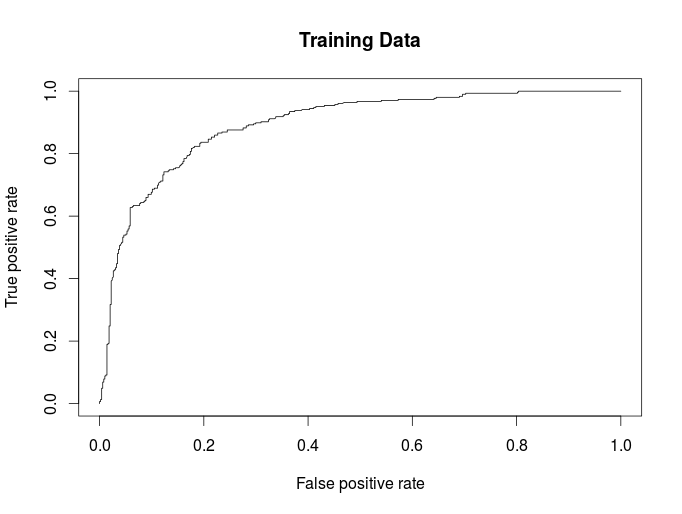
\includegraphics[scale=0.50]{ej1-31.png}
\caption{Curva ROC para cost = 0.001}
\label{}
\end{figure}

\begin{figure}[H]
\centering
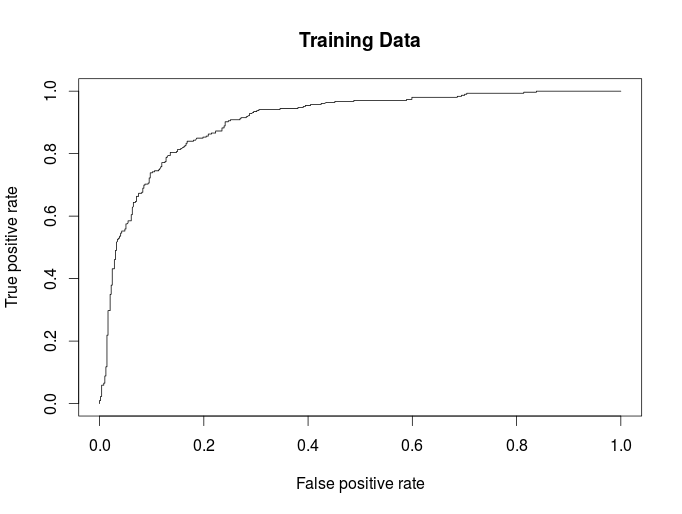
\includegraphics[scale=0.50]{ej1-32.png}
\caption{Curva ROC para cost = 0.01}
\label{}
\end{figure}

\begin{figure}[H]
\centering
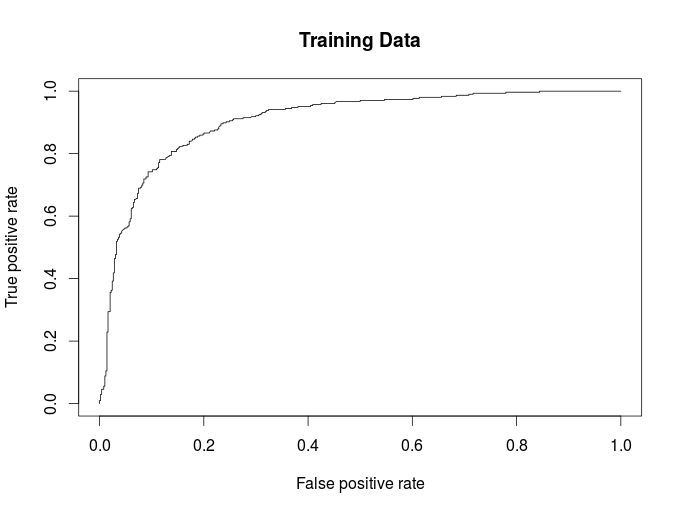
\includegraphics[scale=0.50]{ej1-33.png}
\caption{Curva ROC para cost = 0.1}
\label{}
\end{figure}

\begin{figure}[H]
\centering
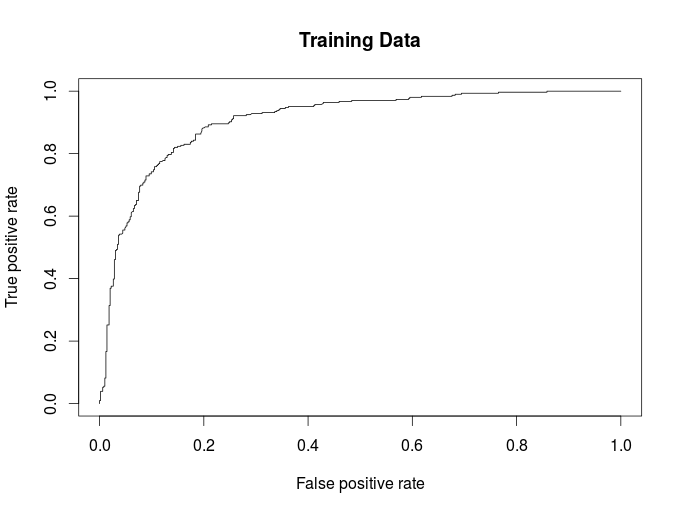
\includegraphics[scale=0.50]{ej1-34.png}
\caption{Curva ROC para cost = 1}
\label{}
\end{figure}

\begin{figure}[H]
\centering
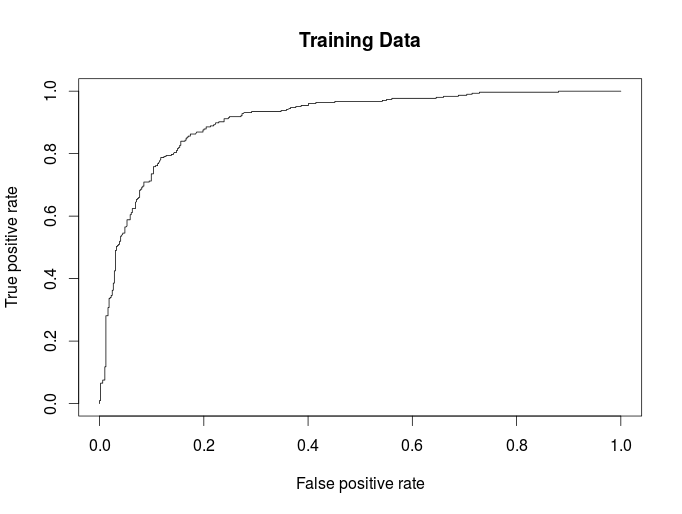
\includegraphics[scale=0.50]{ej1-35.png}
\caption{Curva ROC para cost = 10}
\label{}
\end{figure}

El valor de coste óptimo del parámetro cost es de 0.01, con un rendimiento de 0.175.

Como vemos en las curvas anteriores, si las comparamos con respecto a la calculada para el caso óptimo (cost = 0.01) vemos como esta es más continua (lo que hace que no haya mucha fluctuacion entre los ratios de verdaderos positivos) y por tanto nuestro modelo no nos mostrara valores raros ni saltos de probabiliades, para valores de cost altos la curva crece de forma más ``exponencial''.


\subsubsection{Calcular las tasas de error de “training” y “test” usando el nuevo valor de coste óptimo.}

Ahora nuestros errores han bajado hasta una tasa de error en train del 16,62\% y de test de 18,14\%, por lo que hemos comprobado que el nuevo valor de cost reduce aun mas la probabilidad de error con el nuevo valor óptimo de cost.

\subsubsection{Repetir apartados (2) a (4) usando un SVM con núcleo radial. Usar valores de gamma en el rango [10, 1, 0.1, 0.01, 0.001]. Discutir los resultados}

\begin{figure}[H]
\centering
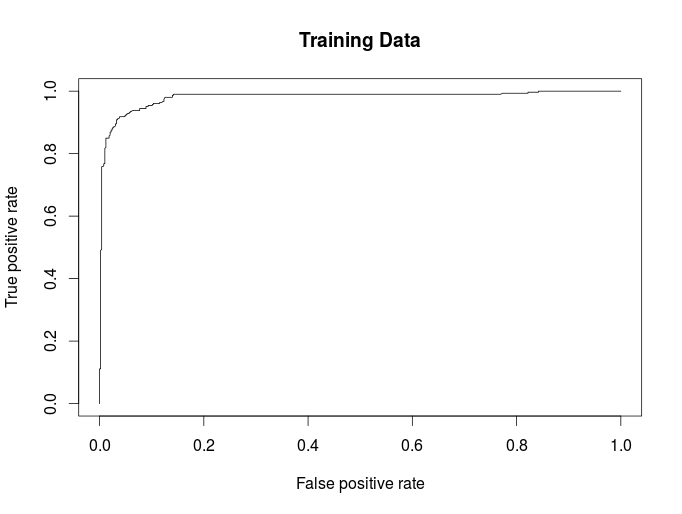
\includegraphics[scale=0.50]{ej1-5.png}
\caption{Curva ROC para gamma = 10}
\label{}
\end{figure}

\begin{figure}[H]
\centering
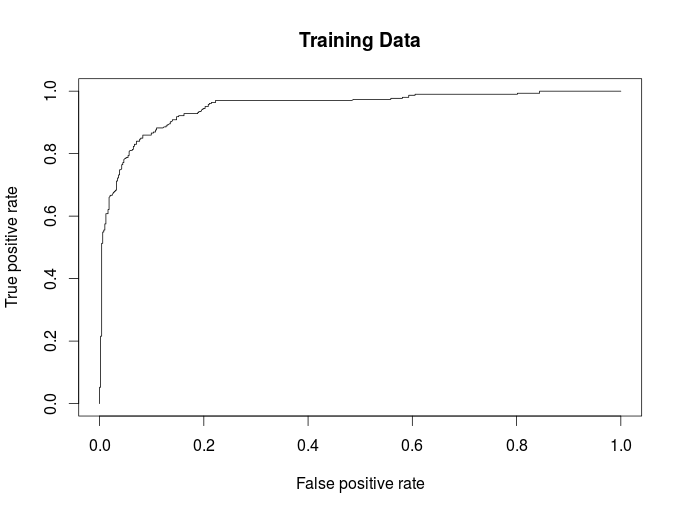
\includegraphics[scale=0.50]{ej1-52.png}
\caption{Curva ROC para gamma = 1}
\label{}
\end{figure}

\begin{figure}[H]
\centering
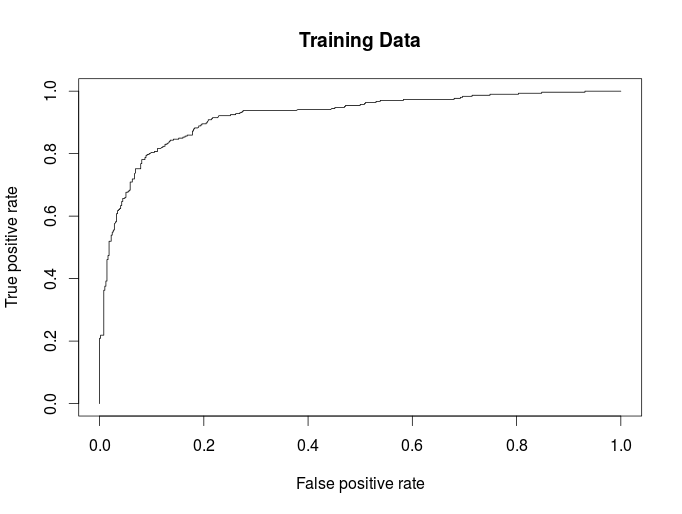
\includegraphics[scale=0.50]{ej1-53.png}
\caption{Curva ROC para gamma = 0.1}
\label{}
\end{figure}

\begin{figure}[H]
\centering
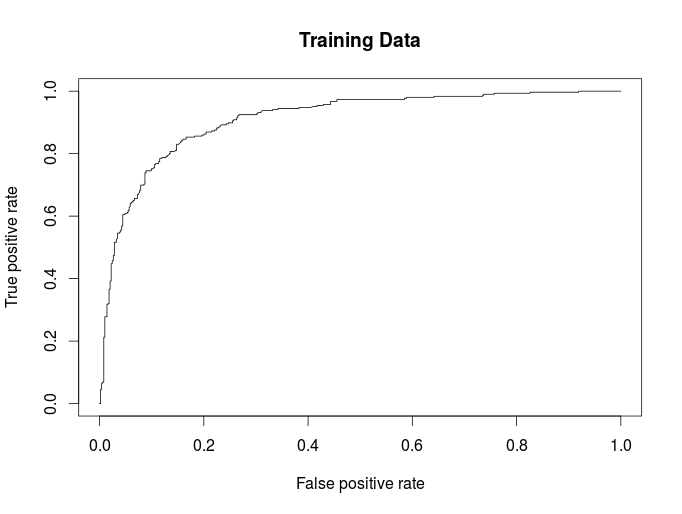
\includegraphics[scale=0.50]{ej1-54.png}
\caption{Curva ROC para gamma = 0.01}
\label{}
\end{figure}

\begin{figure}[H]
\centering
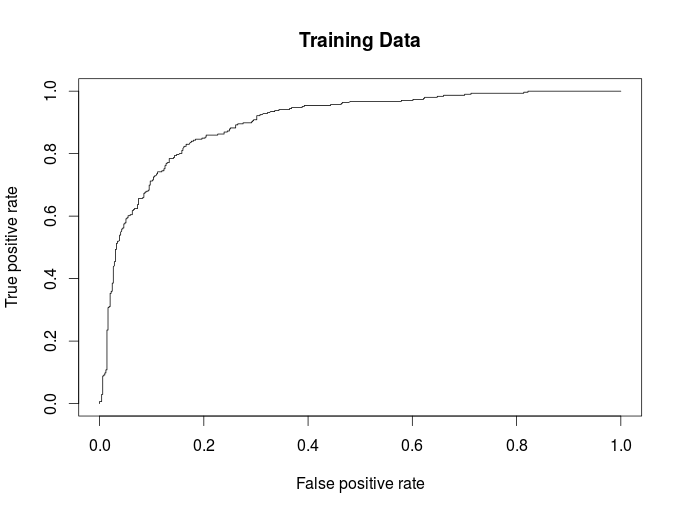
\includegraphics[scale=0.50]{ej1-55.png}
\caption{Curva ROC para gamma = 0.001}
\label{}
\end{figure}

Al principio, con un gamma de valor 10 obtenemos unas tasas de error para training y test de 0.061 y 0.2370 respectivamente. Como podemos ver aunque el error no es muy desorvitado (el de test quiza si, depende de la incertidumbre que asumamos) estan muy descompensados, lo que nos hace inuir que no es un buen valor para el parametro.

Al calcular el valor optimo de gamma R nos dice que es 0.01, por lo que al ajustar el SVM con nucleo radial los errores de training y test se hacen mas proporcionados y por tanto mejores (0.1662 y 0.1814).

Por las razones comentadas en el ejercicio anterior, al comparar las curvas vemos como la que tiene un valor de 0.01 es mejor que el resto.

\subsubsection{Repetir apartados (2) a (4) usando un SVM con un núcleo polinómico. Usar degree con valores 2,3,4,5,6. Discutir los resultados}

\begin{figure}[H]
\centering
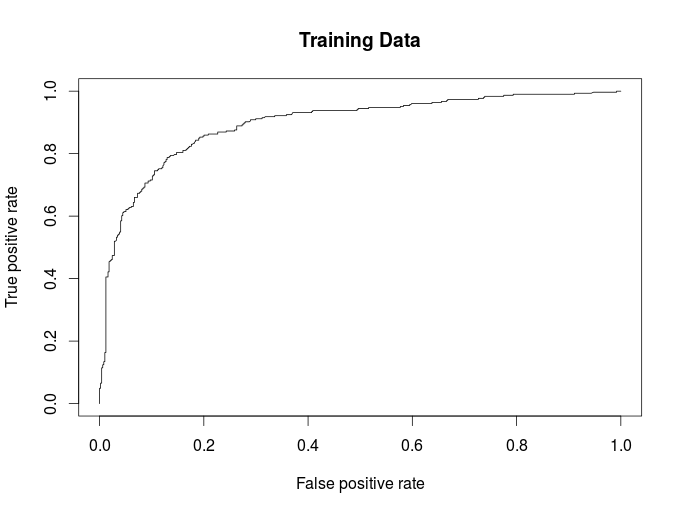
\includegraphics[scale=0.50]{ej1-6.png}
\caption{Curva ROC para degree = 0.001}
\label{}
\end{figure}

\begin{figure}[H]
\centering
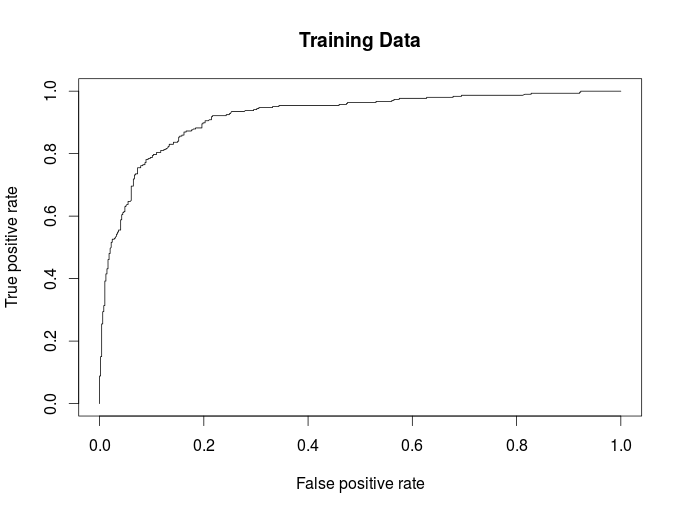
\includegraphics[scale=0.50]{ej1-62.png}
\caption{Curva ROC para degree = 0.001}
\label{}
\end{figure}

\begin{figure}[H]
\centering
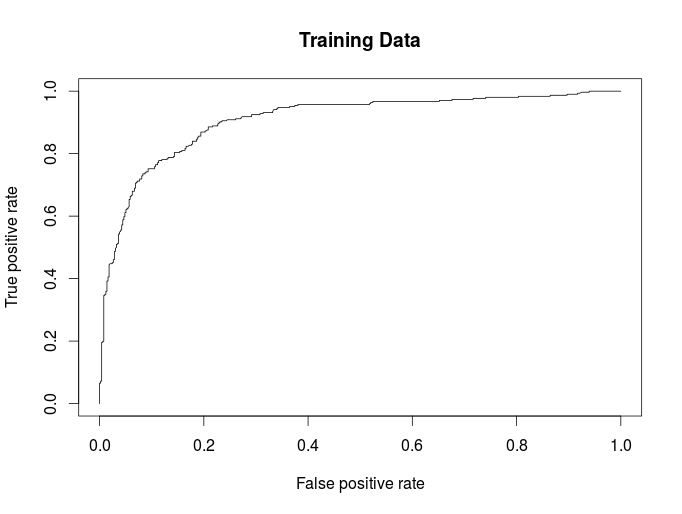
\includegraphics[scale=0.50]{ej1-63.png}
\caption{Curva ROC para degree = 0.001}
\label{}
\end{figure}

\begin{figure}[H]
\centering
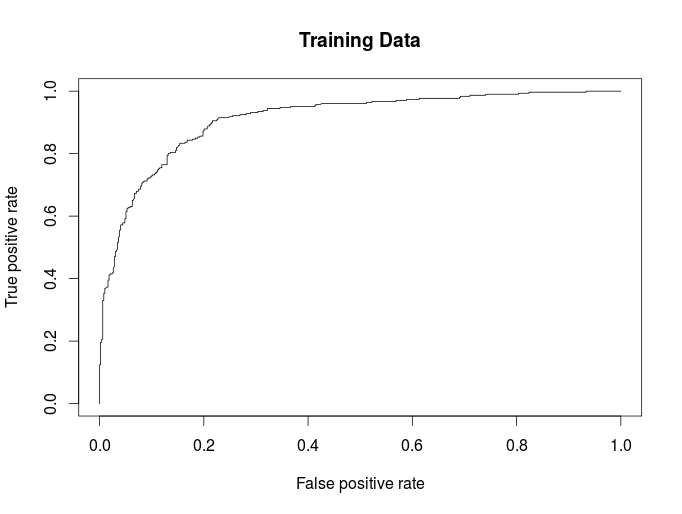
\includegraphics[scale=0.50]{ej1-64.png}
\caption{Curva ROC para degree = 0.001}
\label{}
\end{figure}

\begin{figure}[H]
\centering
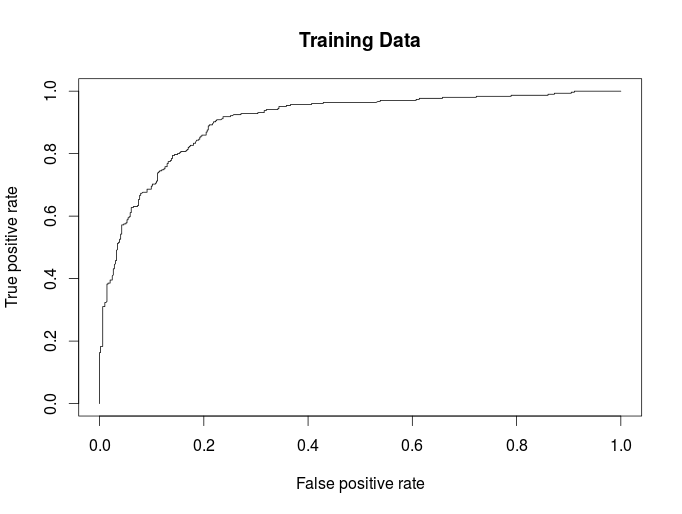
\includegraphics[scale=0.50]{ej1-65.png}
\caption{Curva ROC para degree = 0.001}
\label{}
\end{figure}

Calculado el error de train y test para el primer valor de degree (degree = 2) el modelo nos da buenos valores (0.172 y 0.1888) por lo que o hemos acertado de casualidad a la hora de elegir el valor de degree o el modelo se ajusta mejor a los datos (sin llegar a sobreajustar).

Al calcular el valor óptimo de la variable degree este nos da 3. Nos habiamos aproximado al valor óptimo en el primer calculo pero aun asi se podia acercar mucho mas. Esto ya nos empieza a decir que quiza sea un buen modelo.

Los errores de train y test para degree = 2 son del 14,5\% y 17,03\%. No son valores muy lejanos y a demás son asumibles esos porcentajes de error.

\subsubsection{En global, ¿qué aproximación da el mejor resultado sobre estos datos?}

Teniendo en cuenta la siguiente tabla:\\

\begin{tabular}{lll}
	\textbf{Kernels prámetros opt.} & \% \textbf{Error Train} & \% \textbf{Error test}\\
	Lineal & 16,62 & 18,14\\
	Radial & 16,62 & 18,14\\
	Polinómico & 14,5 & 17,03\\
\end{tabular}\\

Como podemos ver los errores de train y test para los núcleos lineal y radial son los mismos, lo que nos indica que los datos se ajustan de igual manera a ambos nucleos.\\

Además el mejor modelo para usar como clasificador es el polinómico, ya que los errores de train y test bajan sin diferenciarse mucho uno de otro. 

\subsection{Usar el conjunto de datos OJ que es parte del paquete ISLR}

\subsubsection{Crear un conjunto de entrenamiento conteniendo una muestra aleatoria de 800 observaciones, y un conjunto de test conteniendo el resto de las observaciones. Ajustar un árbol a los datos de ``training'', usando ``Purchase'' como la respuesta y las otras variables excepto ``Buy'' como predictores}

\begin{figure}[H]
\centering
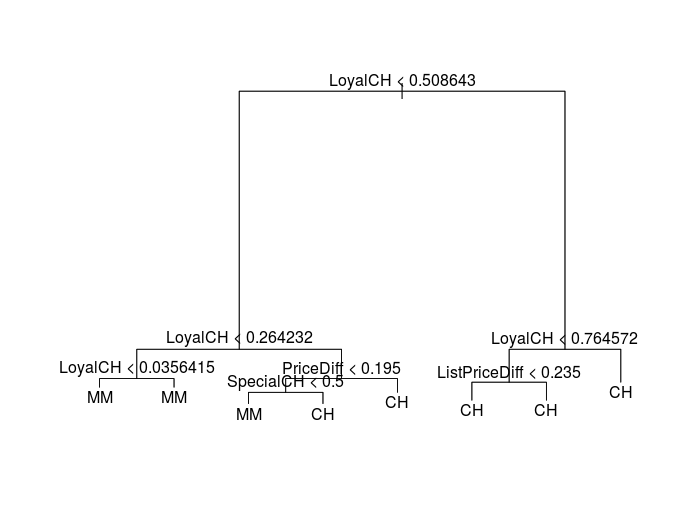
\includegraphics[scale=0.50]{ej2-1.png}
\caption{Árbol de datos de training}
\label{}
\end{figure}

\subsubsection{Usar la función summary() para generar un resumen estadístico acerca del árbol y describir los resultados obtenidos: tasa de error de “training”, número de nodos del árbol, etc. Teclee el nombre del objeto árbol y obtendrá una salida en texto. Elija un nodo e interprete su contenido.}

\begin{figure}[H]
\centering
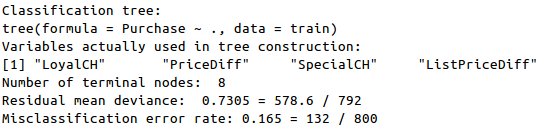
\includegraphics[scale=0.50]{ej2-2.png}
\caption{Árbol de datos de training (summary)}
\label{}
\end{figure}

La función summary nos muestra las variables que se han usado en el arbol, los nodos que este tiene, la desviacion media y el ratio de error de clasificacion.

El arbol no es muy extenso, lo que nos indica que el modelo tiene una complejidad aceptable (solamente 8 nodos). La desviacion media tiene un valor aceptable (0,7305) y un error también asumible (0,165)

Para el nodo 3 por ejemplo R nos muestra la siguiente información:\\

La salida en texto nos da la siguiente información:\\

\textbf{node), split, n, deviance, yval, (yprob)}\\


\textbf{3) LoyalCH > 0.508643 450  318.10 CH ( 0.88667 0.11333 )} \\


El nodo seleccionado es el nodo 3. Si la variable LoyalCH es mayor que 0.5086... seleccionaremos ese nodo,  para expandir, tiene 450 muestras, una desviacion de 318.10 y un valor de y de CH con probabilidad entre 0.8866 y 0.1133.

\subsubsection{Crear un dibujo del árbol. Extraiga las reglas de clasificación más relevantes definidas por el árbol (al menos 4).}

El dibujo del arbol se muestra en el paartado 1 de esta cuestion. En cuanto a las reglas de clasificación mas relevantes:\\

\textbf{1) root 800 1064.00 CH ( 0.6175 0.3825 )  \\
   2) LoyalCH < 0.508643 350  409.30 MM ( 0.2714 0.7286 )  \\
     4) LoyalCH < 0.264232 166  122.10 MM ( 0.1205 0.8795 ) *\\
     5) LoyalCH > 0.264232 184  248.80 MM ( 0.4076 0.5924 )  \\
      10) PriceDiff < 0.195 83   91.66 MM ( 0.2410 0.7590 ) \\ 
        20) SpecialCH < 0.5 70   60.89 MM ( 0.1571 0.8429 ) *\\
        21) SpecialCH > 0.5 13   16.05 CH ( 0.6923 0.3077 ) *\\
      11) PriceDiff > 0.195 101  139.20 CH ( 0.5446 0.4554 ) *\\
   3) LoyalCH > 0.508643 450  318.10 CH ( 0.8867 0.1133 ) *\\}
   
   Estas reglas nos las proporciona R con la función ``misclass''. Esta funcion determina una secuencia de subárboles del árbol recursivamente "cortando" en las divisiones poco importantes.

\subsubsection{Predecir la respuesta de los datos de test, y generar e interpretar la matriz de confusión de los datos de test. ¿Cuál es la tasa de error del test? ¿Cuál es la precisión del test?)}

La matriz de confusión para los datos de test nos muestra que el porcentaje de acierto es medianamente elevado con respecto al conjunto de test (0.7740741). Por otro lado el error de test es de 22,29\%, un poco elevado pero asumible (un 77,40\% de acierto). 

\subsubsection{Aplicar la función cv.tree() al conjunto de “training” para determinar el tamaño óptimo del árbol.}

El tamaño optimo del arbol 4, ya que segun nos indica la salida de cv.tree es àra el que se produce menor desviación.

\begin{figure}[H]
\centering
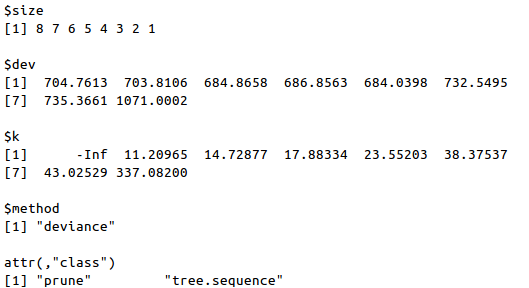
\includegraphics[scale=0.50]{ej2-5.png}
\caption{Salida de cv.tree para el conjunto de training}
\label{}
\end{figure}

\subsubsection{Generar un gráfico con el tamaño del árbol en el eje x y la tasa de error de validación cruzada en el eje y. ¿Qué tamaño de árbol corresponde a la tasa más pequeña de error de clasificación por validación cruzada?}

\begin{figure}[H]
\centering
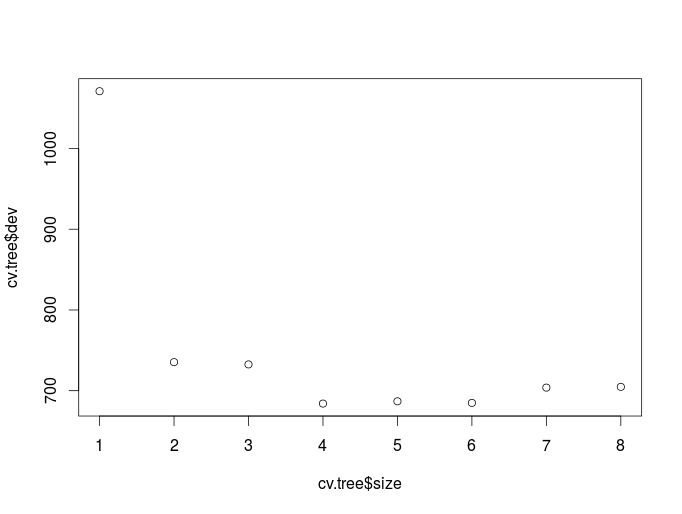
\includegraphics[scale=0.60]{ej2-6.png}
\caption{Gráfico tamaño árbol vs tasa de error VC}
\label{}
\end{figure}

El tamaño del árbol para la tasa mas pequeña de validacion cruzada es el de tamaño 4. Supongo que sera porque en este tamaño habra un compromiso entre tamaño y cantidad de informacion necesaria para que sea un buen modelo.

\subsubsection{Ajustar el árbol podado correspondiente al valor óptimo obtenido en 6. Comparar los errores sobre el conjunto de training y test de los árboles ajustados en 6 con el árbol podado. ¿Cuál es mayor?}
La siguiente tabla representa la comparacion entre los errores de train y test para el árbol podado y sin podar:\\
\begin{tabular}{lll}
	\textbf{Errores} & \textbf{Sin podar} & \textbf{Podado}\\
	\textbf{Train} & 0.165 &  0.165\\
	\textbf{Test} & 0.2259 & 0.2259\\
\end{tabular}

Como podemos ver tanto el erro de train como de test con el arbol podado y sin podar es el mismo, lo que nos indica que en este caso la poda del arbol para el valor óptimo obtenido no es necesaria.

\subsection{Sobre el conjunto de datos Hitters}

\subsubsection{Realizar boosting sobre el conjunto de entrenamiento con 1,000 árboles para un rango de valores del parámetro de ponderación lambda. Realizar un gráfico con el eje x mostrando diferentes valores de lambda y los correspondientes valores de MSE de ``training'' sobre el eje y.}

\begin{figure}[H]
\centering
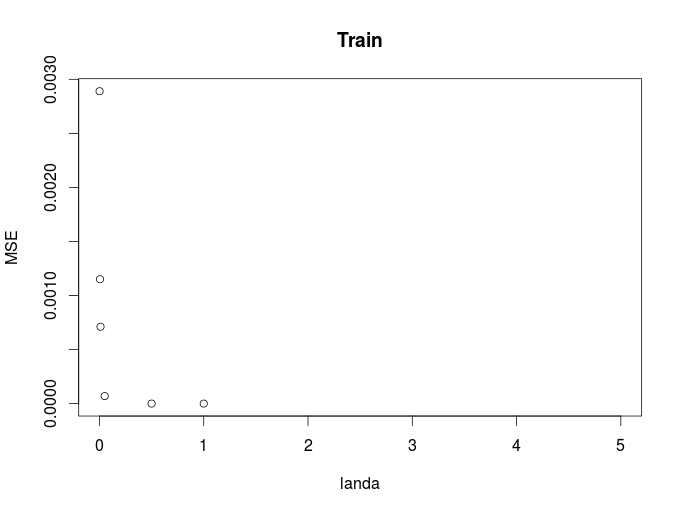
\includegraphics[scale=0.60]{ej3-2.png}
\caption{Gráfico lambda vs MSE trainig}
\label{}
\end{figure}

\subsubsection{Realizar el mismo gráfico del punto anterior pero usando los valores de MSE del conjunto de test. Comparar los valores de MSE obtenidos con boosting para el conjunto test con los obtenidos con los métodos de regresión múltiple y LASSO respectivamente para los mismos datos.}

\begin{figure}[H]
\centering
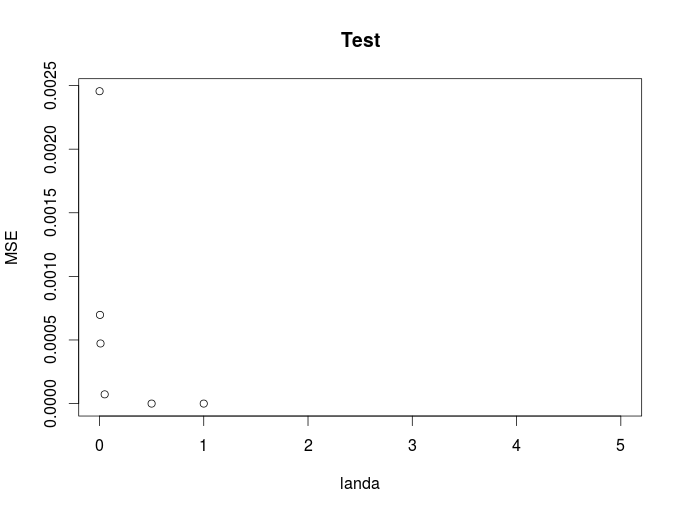
\includegraphics[scale=0.60]{ej3-3.png}
\caption{Gráfico lambda vs MSE test}
\label{}
\end{figure}



\subsubsection{¿Qué variables aparecen como las más importantes en el modelo de ``boosting''?}

Haciendo summary sobre el modelo obtenemos la siguiente grafica:

\begin{figure}[H]
\centering
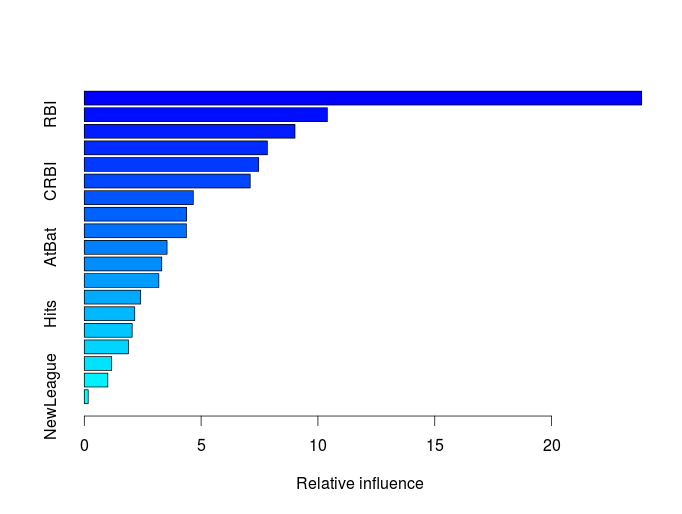
\includegraphics[scale=0.60]{ej3-4.png}
\caption{summary del modelo boosting}
\label{}
\end{figure}

De donde se puede deducir que las variables mas importantes son:

\begin{figure}[H]
\centering
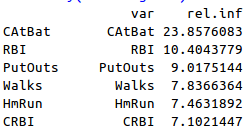
\includegraphics[scale=0.60]{ej4-42.png}
\caption{summary del modelo boosting}
\label{}
\end{figure}

\subsubsection{Aplicar bagging al conjunto de ``training'' y volver a estimar el modelo. ¿Cuál es el valor de MSE para el conjunto de test en este caso?}

El valor MSE es de  0.1195, lo que quiere decir que la diferencia entre el estimador y lo que se estima es muy baja debido a que el estimador tiene en cuenta la información que puede producir una estimación más precisa. Aunque este no sea exactamente 0 (se deberá a la aleatoriedad de las muestras), lo es a efectos prácticos.







\end{document}